\documentclass[tikz,border=0pt]{standalone}
\usepackage{amsmath,amssymb}
\usetikzlibrary{calc,decorations.pathreplacing}

\definecolor{ink}{HTML}{0B1020}
\definecolor{paper}{HTML}{F4F1EA}
\definecolor{muted}{HTML}{AAB7C4}
\definecolor{cyan}{HTML}{4FD1E8}
\definecolor{violet}{HTML}{A78BFA}
\definecolor{amber}{HTML}{F6C453}
\definecolor{gridline}{HTML}{24334C}

\begin{document}
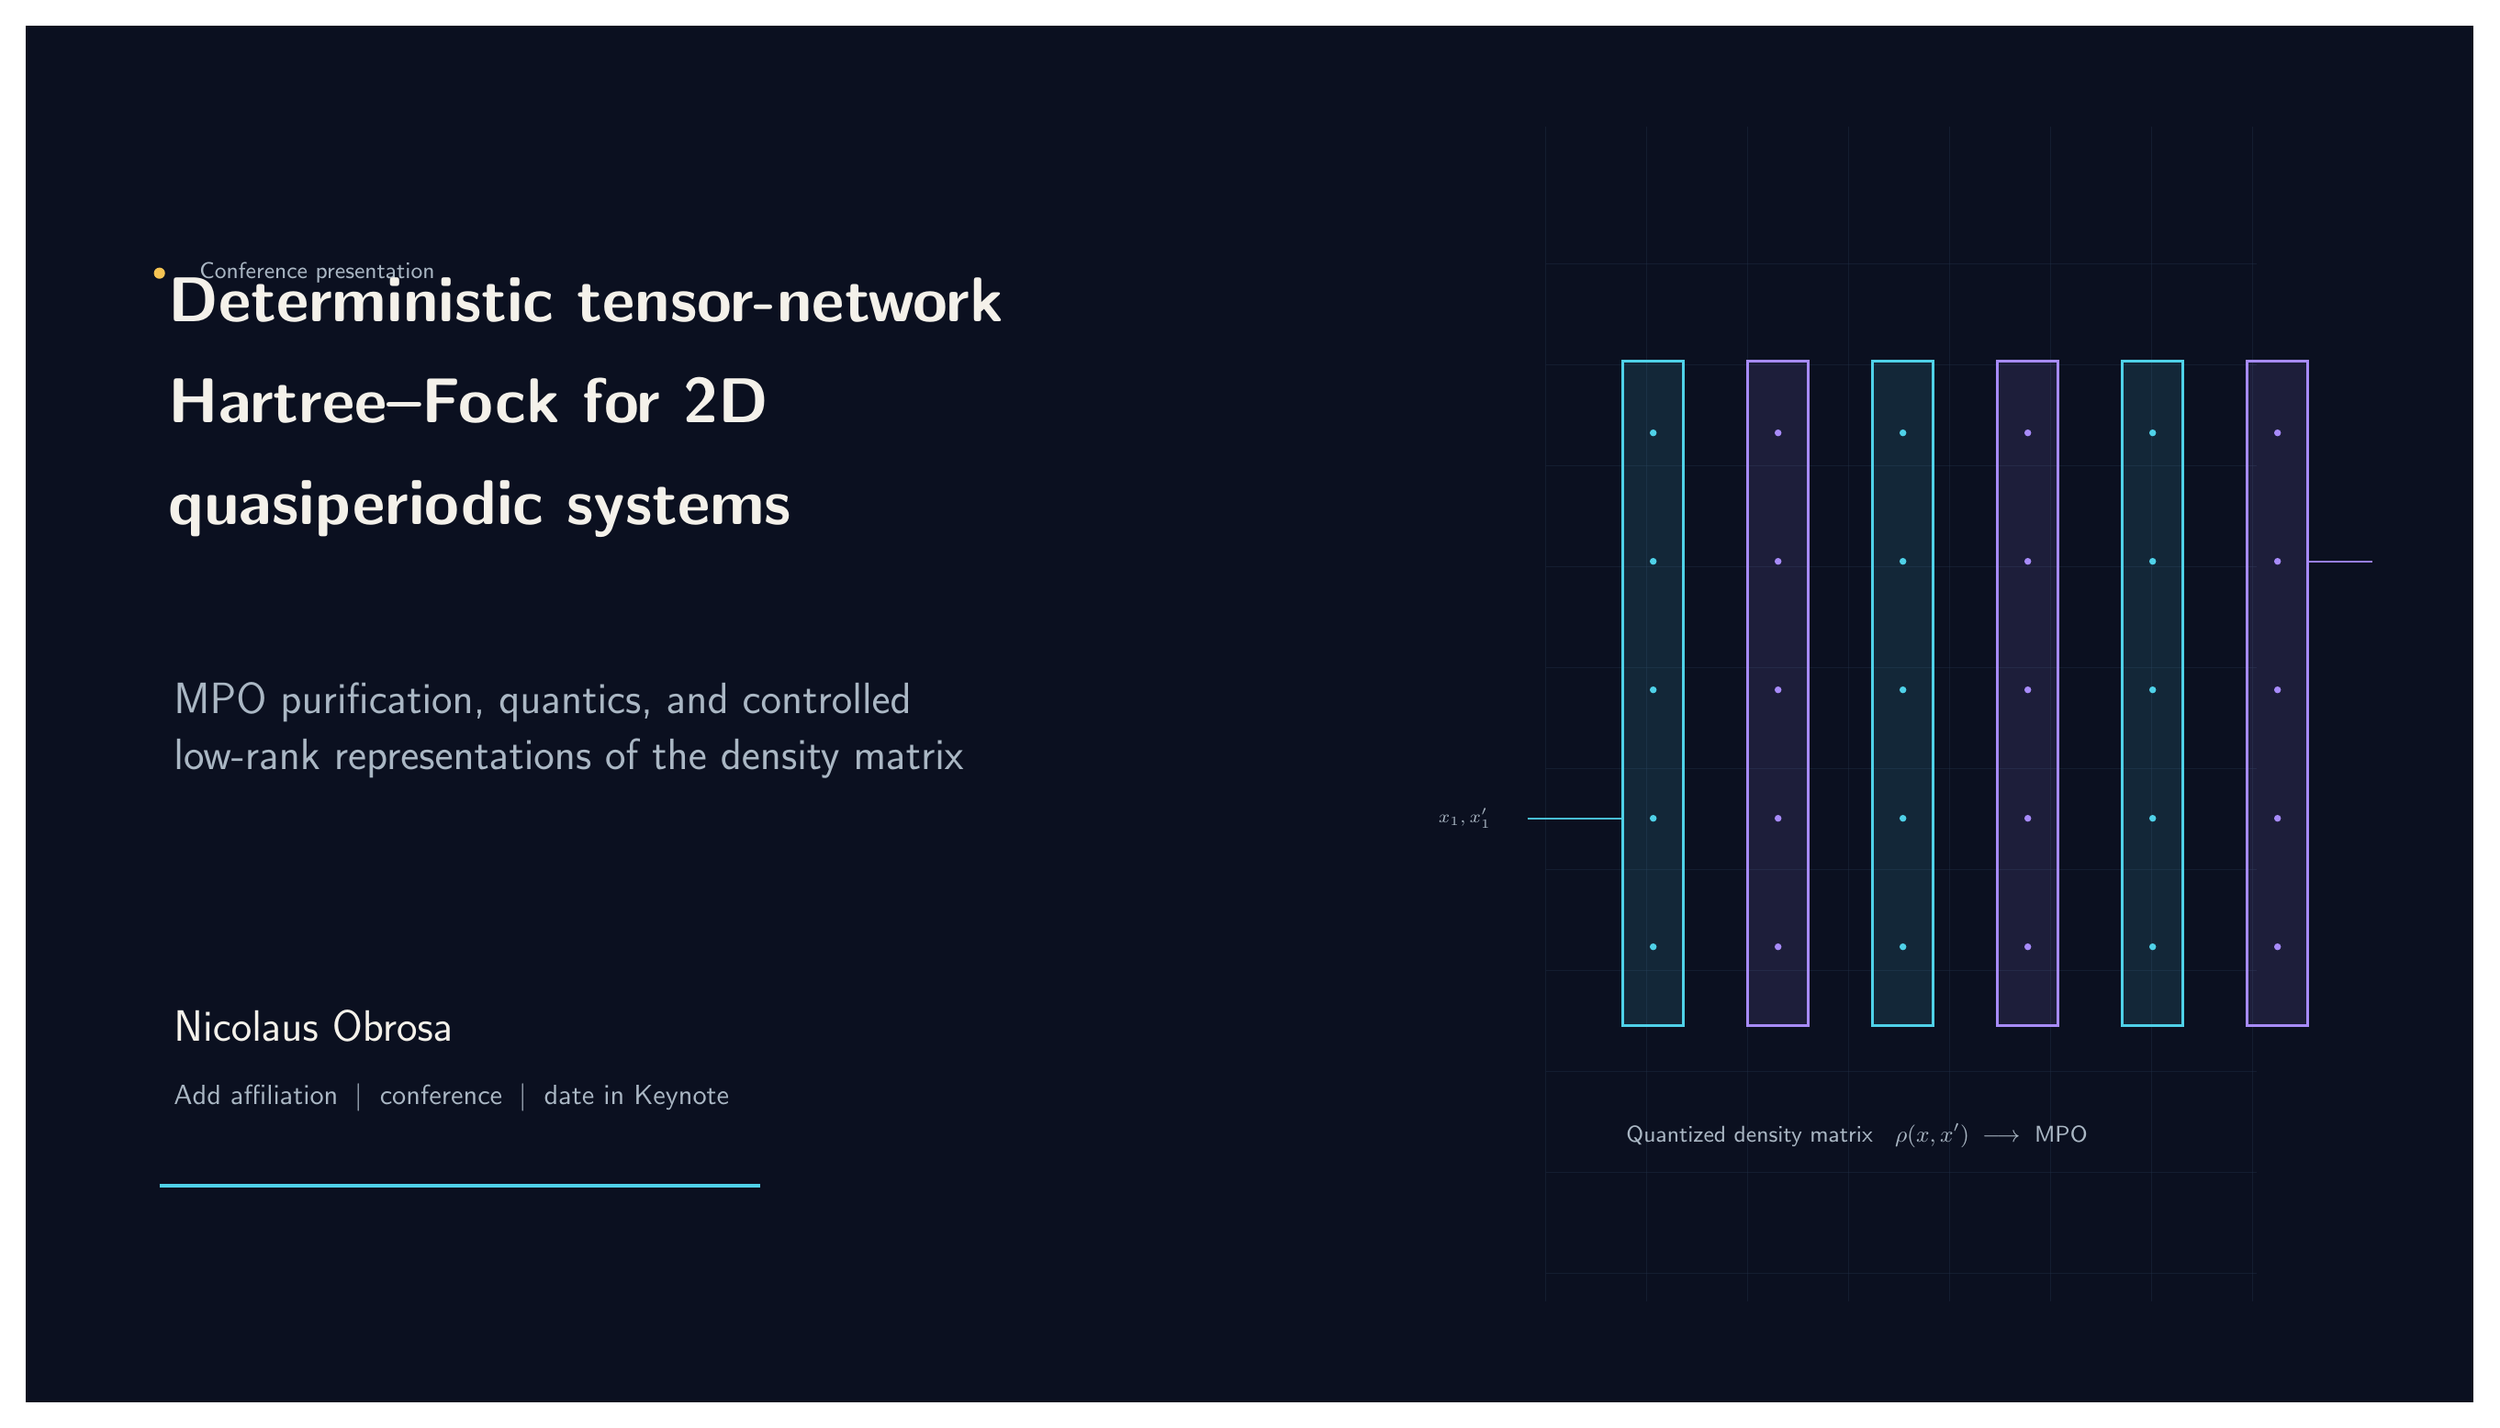
\begin{tikzpicture}[x=1in,y=1in]
  \path[fill=ink] (0,0) rectangle (13.3333,7.5);

  % Subtle quantics grid in the right background.
  \foreach \i in {0,...,7}
    \draw[gridline,opacity=.38,line width=.25pt] (8.28+\i*.55,.55) -- (8.28+\i*.55,6.95);
  \foreach \i in {0,...,10}
    \draw[gridline,opacity=.38,line width=.25pt] (8.28,.70+\i*.55) -- (12.15,.70+\i*.55);

  % MPO cores: the deliberately simple visual motif on the right.
  \foreach \x/\c in {8.70/cyan,9.38/violet,10.06/cyan,10.74/violet,11.42/cyan,12.10/violet} {
    \path[fill=\c,opacity=.12] (\x,2.05) rectangle +(0.33,3.62);
    \draw[\c,line width=1.2pt] (\x,2.05) rectangle +(0.33,3.62);
    \foreach \y in {2.48,3.18,3.88,4.58,5.28}
      \fill[\c] (\x+.165,\y) circle (1.35pt);
  }
  \draw[cyan,line width=.65pt,opacity=.9] (8.18,3.18) -- (8.70,3.18);
  \draw[violet,line width=.65pt,opacity=.9] (12.43,4.58) -- (12.78,4.58);
  \node[anchor=east,text=muted,font=\sffamily\scriptsize] at (8.03,3.18) {$x_1,x'_1$};
  \node[anchor=west,text=muted,font=\sffamily\small] at (8.67,1.45)
    {Quantized density matrix \; $\rho(x,x')\;\longrightarrow\;$ MPO};

  % Fine terminal-line and accents.
  \draw[cyan,line width=1.4pt] (.73,1.18) -- (4.00,1.18);
  \fill[amber] (.73,6.15) circle (2.2pt);
  \node[anchor=west,text=muted,font=\sffamily\small] at (.90,6.15)
    {Conference presentation};

  % Main textual hierarchy.
  \node[anchor=west,text=paper,font=\sffamily\bfseries\fontsize{35}{40}\selectfont,align=left] at (.73,5.42)
    {Deterministic tensor-network\\Hartree--Fock for 2D\\quasiperiodic systems};
  \node[anchor=west,text=muted,font=\sffamily\fontsize{16}{22}\selectfont,align=left] at (.76,3.66)
    {MPO purification, quantics, and controlled\\low-rank representations of the density matrix};
  \node[anchor=west,text=paper,font=\sffamily\fontsize{16}{20}\selectfont] at (.76,2.05)
    {Nicolaus Obrosa};
  \node[anchor=west,text=muted,font=\sffamily\fontsize{11}{16}\selectfont] at (.76,1.66)
    {Add affiliation \;\textbar\; conference \;\textbar\; date in Keynote};
\end{tikzpicture}
\end{document}
